
%Intro CHECKED!!


\chapter{Introducción}
\label{chap1:intro}


\section{Contexto General}
\label{chap1:CG}

Entre 1989 y 1990, Tim Berners-Lee acuñó el concepto de \textit{World Wide Web} y con ésto realizó la construcción del primer \textit{Web Server}, \textit{Web Browser} y las primeras páginas \textit{Web}. Mucho antes que aparecieran los grandes sistemas que ahora conocemos, el \textit{Web Browser} permitía navegar páginas estáticas y realizar una serie de acciones limitadas a las tecnologías de ese tiempo. En la actualidad el \textit{browser} es la herramienta predilecta por todos, desde comprar tickets para una película, realizar reuniones por videoconferencia y muchas otras tareas que invitan a nuevas formas de interactuar y comunicar.

Durante la conocida \textit{guerra de navegadores}, en la década de los noventa, los \textit{browser} tuvieron solo el objetivo de poder adquitir la mayor cantidad de usuarios posibles, entregando mejores funcionalidades que sus competidores. Debido a esto era habitual encontrar muchos parches que solucionaban problemas de seguridad, dada la cantidad de errores de programación y deficiente estructura del navegador, dado que no había una pronta preocupación por integrar Seguridad en el Software. Además la nula documentación que existía debido a la gran competitividad, muchas veces hacía que las extensiones hechas por \textit{third-parties} creaban más agujeros de seguridad, que nuevas funcionalidades. El inicio del Software Libre u \textit{Open Source}, cambió el escenario y las circunstancias, pero aún así, existen navegadores propietarios que no exponen la arquitectura de sus aplicaciones.

En el último tiempo el mercado de los \textit{Web Browser} ha crecido bastante (Figura \ref{fig:UsageShare}), principalmente debido a la robustez que éstos poseen y a la cantidad de años que llevan desarrollándose en la industria de Software. Los navegadores más conocidos son: Google Chrome o su versión Open Source Chromium, Firefox, Internet Explorer, Opera y Safari; siendo los primeros 3 el enfoque de este trabajo.

    \begin{figure}[h]
        \centering
        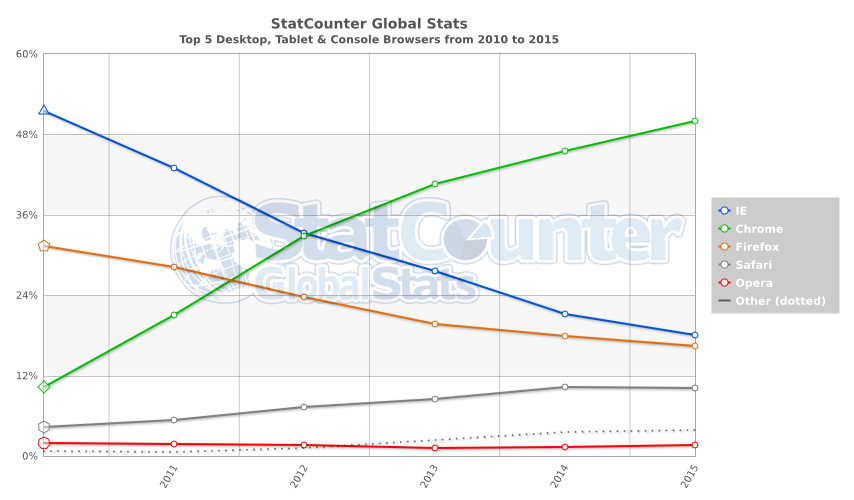
\includegraphics[width=1\textwidth]{figures/StatCounter-browser-ww-yearly-2010-2015.png}
        \caption{Porcentaje de uso de Navegadores. Fuente: \cite{statBrow}}
        \label{fig:UsageShare}
    \end{figure}

La \textit{Web 2.0} se inició con el uso intensivo de tecnologías como AJAX, y ésto ha permitido una nueva simbiosis entre el usuario, el Web Browser y el Servidor o Web Server que se comunican entre sí. El Navegador Web es una herramienta indispensable para todo tipo de tareas computacionales como comunicacionales, su existencia ha penetrado completamente en las labores diarias de todos nosotros. En este mismo instante, la Web a evolucionado nuevamente obteniendo un nuevo nombre: \textit{Web 3.0}, donde se realiza el uso de inteligencia artificial y sistemas de recomendación para generar nuevos tipos de contenido para el usuario.


\section{El Problema: Desarrollo de Software y Seguridad}
\label{chap1:SD_SS}

Ningún Desarrollo de Software es igual al anterior. Por cada nuevo proyecto que surge es necesario ver qué tipo de proceso es el que se usará, qué personas serán parte del grupo de trabajo, qué condiciones económicas estará expuesto, qué \textit{Stakeholder} están pendientes de que el Proyecto salga exitoso y un sin número de variables, no menos importantes a considerar. Por lo tanto, dependiendo de lo anterior, los sistemas podrían llegar a ser simples o muy complejos. En consecuencia, se hace necesario tener ciertas metodologías que aseguren que se cumplan con todos los Requerimientos Funcionales como No-Funcionales del Sistema a construir. Sin embargo, un problema que existe recurrentemente, es que la mayoría del Software construído contiene numerosos \textbf{defectos} y \textbf{errores}, generando así \textbf{vulnerabilidades} que son encontradas y explotadas por los atacantes, generando un compromiso parcial o total del sistema \cite{goertzel2007software}. Lo anterior sucede frecuentemente por que los sistemas no son desarrollados teniendo en cuenta la seguridad \cite{Yoder1998, fernandez2004methodology, WhyteHarrison}.

Muchas veces al desarrollar sistemas, se prefiere utilizar API's\footnote{Application Programming Interface} de otros sistemas para poder incluir funcionalidades ya implementadas, fomentando así el Reuso de piezas de Software. Si bien lo anterior es una buena práctica, si el sistema no cuenta con las medidas de seguridad necesarias, estas piezas podrían ser causa de amenazas de seguridad que terminarían por corromper el sistema y en consecuencia podría causar una pérdida monetaria a los \textit{Stakeholders}. Lo expuesto anteriormente ejemplifica perfectamente con lo que tienen que lidiar los equipos de trabajo en proyectos de Desarrollo de Software, cuando dentro de sus preocupaciones la seguridad queda como un trabajo extra y no como parte del desarrollo completo. 

Bien es sabido que un proyecto en producción que presente problemas que involucren a varias entidades, el costo asociado puede llegar a ser altísimo \cite{cert}, sin olvidar que podría llegar a afectar la Confidencialidad, Integridad y Disponibilidad de los datos de los involucrados con el sistema  \cite{interCoursera}. Por esto mismo, es imperante que sean entendidos, desde el comienzo, las preocupaciones de los \textit{Stakeholders} y los Requerimientos de Seguridad asociados, y que adémás todos los involucrados los entiendan perfectamente. Según \cite{WhyteHarrison}, la falta de preocupación en temas de seguridad en desarrollos de software no tiene una raíz principal, sino diversos factores como: la falta de estudios de seguridad en las mallas curriculares de las Universidades, pocos fondos para la investigación, la falta de iniciativa y preocupación desde la industria, el exceso de confianza de los desarrolladores, etc., son los causantes de las futuras vulneraciones en sistemas críticos. 

La literatura que habla de la construcción de \textit{Secure Software} o Software Seguro, indica que los practicantes de Desarrollo de Software deben entender, en gran medida, los problemas de seguridad que podrían llegar a ocurrir en sus sistemas. No basta con saber cómo unir las piezas, no basta con que cada pieza de por si sea segura, si los componentes del sistema no actuan de forma coordinada, probablemente éste no será seguro \cite{fernandez2013security}, dado que la seguridad es una Propiedad Sistémica que necesita ser vista de manera holística y al inicio del proceso.

Un sistema cualquiera conectado a Internet y accedido por un usuario a través de un Navegador, estará en algún momento de su vida útil bajo amenazas que el Desarrollador debe estar al tanto. Al conocer las amenazas es posible comunicar a los \textit{Stakeholders}, de los posibles peligros a los que se enfrentan, aún cuando en el equipo de Desarrolladores no exista un experto en seguridad. Bajo esta misma lupa, una Arquitectura de Referencia permitiría comunicar efectivamente los componentes, interacciones y comportamientos existentes entre el \textit{browser} y el sistema con el que se comunica, de tal manera que sería posible entender mejor los posibles problemas de seguridad que el \textit{Browser} puede llegar a generar. 

\section{Motivación: ¿Por qué estudiar el Browser?}
\label{chap1:motiv}

Con la aparición de la \textit{Web 2.0 y 3.0}, con el uso de \textit{AJAX}, inteligencia artificial y sistemas de recomendación, permitieron nuevas formas de interacción entre usuarios y sistemas, lo que causó que el \textit{browser} fuera usado extensivamente en los nuevos Desarrollos de Software, dado que:
\begin{itemize}
	\item Permite disminuir los costos de construir un programa Cliente (desde cero) para el usuario del sistema.
	\item Actualmente la Seguridad implementada que los \textit{Web Browser} es bastante buena, dado que existen grandes compañias se aseguran de ello (Google, Microsft, Mozilla entre las más conocidas). 
	\item El \textit{browser} es una herramienta indispensable. La mayoría de los sistemas que lo usan en la vida cotidiana son de tipo: \textit{online banking}, declaración de impuestos, promoción de empresas o tiendas, compras, y mucho más.
\end{itemize}

Sin embargo los sistemas que dependen del uso del \textit{Browser}, deben de tener en cuenta las posibles amenazas de seguridad a las que se enfrentarán por el solo hecho de usarlo. Para un proyecto de gran envergadura, sería un error no tener en consideración los posibles peligros que trae el uso del \textit{Browser}, y es el deber de todo integrante del equipo de Desarrollo tener el conocimiento de la seguridad del Cliente Web. El entendimiento de la estructura subyacente del Web Browser podría asegurar que las personas que trabajen en el desarrollo, comprendan los \textit{trade-off} al momento de diseñar un Software que necesite la colaboración del Navegador Web \cite{535061, 2005-grosskurth-browser-refarch,preprint-grosskurth-browser-archevol}; poniéndolo de otra forma, un atacante es capaz de explotar un ataque en el sistema, dado que tiene el conocimiento subyacente del \textit{Browser}, conoce sus vulnerabilidades y mecanismos de defensa.

En \cite{goertzel2007software, WhyteHarrison} mencionan que la cantidad de tiempo dedicado en temas de seguridad, por los estudiantes en áreas de la Información/Computación/Software es casi nula. Si bien existen diversos factores \cite{WhyteHarrison} que pueden ser causa de este comportamientos, principalmente las universidades y las industrias son un fuerte factor en la adopción de un cambio de mentalidad. Desarrollar un sistema crítico (o no) pero seguro, representa un gran desafío. No solo para los desarrolladores, si no también para los involucrados indirectamente, como los usuarios que navegan con un \textit{browser} para hacer uso de éste sistema. Por lo mismo, es entendible que la seguridad sea un tema complicado de impartir, pero eso no significa que sea imposible. Nuestro trabajo tiene la intención de presentar un marco conceptual, que permita entender más este atributo de calidad y que pueda ayudar a otros desarrollos ser más seguros.

Este trabajo tiene una motivación principal. Ésta es ayudar a quien lo necesite con el conocimiento necesario para entender el funcionamiento y construcción del Cliente, el Web Browser, los beneficios detrás de la Seguridad implementada en el \textit{Browser} y de los peligros existentes de los que nos protegen. De esta manera se espera que alguien que lea este trabajo, tanto Estudiantes como Desarrolladores de Software, obtengan el conocimiento necesario al momento de trabajar junto con el Navegador Web al realizar un Desarrollo de Software que dependa de éste.

De nuestro conocimiento hasta el momento, no existe ninguna propuesta de Arquitectura de Referencia del \textit{Browser} moderno, solo existe material desactualizado que no se adecua al paisaje actual \cite{2005-grosskurth-browser-refarch}. Creemos que una falta de conocimientos de seguridad con respecto al \textit{Browser}, podría afectar de forma directa el desarrollo de aplicaciones que lo utilizan. Por esto mismo, una guía o compilado de información, semi-formal, que una los conceptos y componentes, como lo hace una Arquitectura de Referencia, podría enseñar a desarrolladores no expertos en seguridad, los peligros que existen. Nuestro trabajo considera a la seguridad como una propiedad sistémica que debe ser tomada en cuenta desde el inicio de su desarrollo \cite{fernandez2004methodology, fernandez2006defining, braz2008eliciting, fernandez2013security, Fernandez2011}.


\section{Contribuciones}
\label{chap1:contr}

Dada la falta de documentación para enseñar a desarrolladores no expertos en seguridad, acerca de los componentes, interacciones y comportamientos del Web Browser, el \textbf{Objetivo General} de esta Memoria es: Generar un cuerpo organizado de información sobre el Web Browser y su Seguridad, de tal manera que se pueda sistematizar, organizar y clasificar el conocimiento adquirido en un documento, con formato semi-formal, tanto para Profesionales como Estudiantes del área Informática que estén insertos en el área de Desarrollo de Software.

Este trabajo busca cumplir con los siguientes \textbf{Objetivos Específicos}:

\begin{itemize}
	\item Comprender los conceptos relacionados al navegador web, sus componentes, interacciones o formas de comunicación, amenazas y ataques a los que puede estar sometido, como también los mecanismos de defensa. Esto se realizará a través del desarrollo de un Estado del Arte sobre el Browser.
	\item Identificar actores, componentes, funciones, relaciones, requerimientos y restricciones del Navegador, para lograr abstraer una Arquitectura de Referencia (AR) a partir de documentación disponible en Internet, blogs de desarrolladores, papers e iniciar un pequeño catálogo de Patrones de Mal Uso. Esto permitirá condensar el conocimiento obtenido en el punto anterior a través de documentos semi-formales, lo que permitirá generar una guía para comunicar los conceptos relevantes que pudieran afectar la relación existente entre un desarrollo de software y el navegador.
	\item Profundizar el conocimiento en ataques relacionados con métodos de Ingeniería Social.
	
\end{itemize} 

Particularmente se ha escogido como metodología base la dada por Fernandez\cite{braz2008eliciting,fernandez2013security}. Una Arquitectura de Referencia (AR) tiene como objetivo el mismo descrito en \cite{2005-grosskurth-browser-refarch, preprint-grosskurth-browser-archevol, Avgeriou2003, Galster2011a}, éste es capturar la esencia de la arquitectura a través de una colección de sistemas similares, por medio del reuso arquitectónico, y además ayudar a los \textit{implementors} o desarrolladores del software, a entender los \textit{trade-off} cuando se diseñan nuevos sistemas, y puede ayudar a los mantenedores de estos sistemas a entender el código \textit{legacy} usado. Una Arquitectura de Referencia permite además comparar las diferencias en decisiones de diseño del Navegador y así poder entender los cambios realizados a lo largo del Desarrollo de un sistema. Junto con lo anterior, ĺa AR permitirá tener una visión holística del sistema y mostrará las decisiones de alto nivel para asegurar la Seguridad del sistema. 

Por otra parte, los Patrones de Mal Uso o Uso Indebido, permitirán enseñar y comunicar las posibles formas en que tal sistema puede ser usado inapropiadamente.

En este trabajo se presentará nuestra Arquitectura de Referencia y un Patrones de Uso Indebido, que usarán la AR construida para mostrar los componentes y mensajes que una amenaza puede realizar, con tal de lograr un ataque en el \textit{Browser}. El uso de patrones nos permitirá abstraer componentes y comunicaciones entre dichos sistemas, al mismo tiempo que vislumbrará los mecanismos de seguridad implementados. Los patrones son herramientas de gran valor, que permiten generar el entendimiento de los aspectos funcionales y pueden complementar con otros patrones relacionados para alcanzar una arquitectura más entendible. Estos patrones serán presentados usando el template POSA \cite{buschman1996system} y UML, para así modelar las interacciones entre los diversos componentes de la arquitectura.

\section{Metodología}
\label{chap1:Met}
Este trabajo se realizará de la siguiente forma:
\begin{enumerate}
	\item Introducción de un \textit{Framework conceptual} para entender los conceptos relacionados.
	\item Hablar sobre las (in)seguridades en el Browser, a través de los posibles ataques que se pueden dar en el Browser y cómo éstos pueden afectar a los sistemas que lo usan.
	\item Presentar un Estado del Arte sobre el \textit{Browser}, sobre las distintas arquitecturas, lo que se ha hecho en Arquitecturas de Referencia en el Browser, o patrones relacionados a éste.
	\item Identificar los conceptos, actores, componentes, interacciones y funciones, para poder generar una Arquitectura de Referncia del Browser. Con esto se construirá patrones de arquitectura que definan los componentes y responsabilidades.
	\item Construir patrones de Mal Uso/Uso Indebido por medio del punto anterior.
\end{enumerate}

\section{Estructura del Documento}
\label{chap1:estruct}

El presente documento trata del trabajo de Memoria, que se divide en las siguientes partes:

\begin{itemize}
	\item En el capítulo \ref{chap2:FC} se presenta un \textit{framework conceptual} los conceptos de seguridad básicos que hay que entender en este trabajo.
	\item Luego de tener un extenso conocimiento de lo que actualmente es conocido como \textbf{Web Browser}, el capítulo \ref{chap3:MT} presenta un marco teórico de la (in)seguridad del Browser donde se verán los posibles ataques que se puedan dar a esta pieza de software.
	\item En el capítulo \ref{chap4:EA} se presenta el Estado del Arte de las propuestas de Arquitecturas de Referencias o similares sobre el Web Browser, así como la existencia de los Browser más usados y Patrones existentes. Además una descripción de los componentes más importantes en cada Navegador es entregada.
	\item La Arquitectura de Referencia, nuestra propuesta, se presenta en el capítulo \ref{chap5:ArqRefWB}. Esta presenta la abstracción de las propuestas vistas en el capítulo \ref{chap4:EA}.
	\item Previo a la construcción del Patrón de Mal Uso en el capítulo \ref{chap6:Misuse}, se analizarán las amenazas que existen en el Browser a través de la AR construída. 
	\item Finalmente se presentarán las Conclusiones sobre el trabajo realizado y se presentará posibles trabajos a futuro sobre este mismo tema.
\end{itemize}












